\documentclass[11pt]{article}

\usepackage[margin=1in]{geometry}
\usepackage[T1]{fontenc}
\usepackage{lmodern}
\usepackage{microtype}
\usepackage{amsmath,amssymb,amsthm,mathtools}
\usepackage{mathrsfs}
\usepackage[dvipsnames]{xcolor}
\usepackage[most]{tcolorbox}
\usepackage{tikz}
\usetikzlibrary{decorations.markings,patterns}
\usepackage{enumitem}
\usepackage{tocloft}
\usepackage[hidelinks]{hyperref}

\definecolor{courseblue}{HTML}{1F4E79}
\definecolor{lightblue}{HTML}{EAF2F8}
\definecolor{lightgreen}{HTML}{EAF7EA}
\definecolor{lightpink}{HTML}{FCE8EF}
\definecolor{lightyellow}{HTML}{FFF8D6}
\definecolor{warningyellow}{HTML}{D6A000}
\definecolor{exercisebg}{HTML}{FDEAEA}
\definecolor{exerciseframe}{HTML}{B54040}
\definecolor{examplebg}{HTML}{F4FAFE}
\definecolor{exampleframe}{HTML}{85C1E9}
\definecolor{darkgray}{HTML}{333333}
\definecolor{lightorange}{HTML}{FDEBD8}
\definecolor{orangeframe}{HTML}{E08A3C}
\definecolor{remarkbg}{HTML}{F3EEFB}
\definecolor{remarkframe}{HTML}{9B7FC9}

\setlength{\parindent}{0pt}
\setlength{\parskip}{0.65em}
\setlist[itemize]{topsep=0.25em,itemsep=0.15em}
\renewcommand{\cftsecleader}{\cftdotfill{\cftdotsep}}
\renewcommand{\cftsubsecleader}{\cftdotfill{\cftdotsep}}

\theoremstyle{plain}
\newtheorem{theorem}{Theorem}[section]
\newtheorem{proposition}[theorem]{Proposition}
\newtheorem{lemma}[theorem]{Lemma}
\newtheorem{corollary}[theorem]{Corollary}
\theoremstyle{definition}
\newtheorem{definition}[theorem]{Definition}
\newtheorem{example}[theorem]{Example}
\newtheorem{exercise}[theorem]{Exercise}
\theoremstyle{remark}
\newtheorem*{remark}{Remark}
\newtheorem*{fact}{Fact}
\newtheorem*{warning}{Warning}

\tcolorboxenvironment{definition}{
  enhanced,
  unbreakable,
  colback=lightgreen,
  colframe=ForestGreen,
  boxrule=0.7pt,
  arc=2pt,
  left=6pt,
  right=6pt,
  top=5pt,
  bottom=5pt
}

\tcolorboxenvironment{remark}{
  enhanced,
  colback=remarkbg,
  colframe=remarkframe,
  before upper={\setlength{\parskip}{0.5em}},
  boxrule=0.7pt,
  arc=2pt,
  left=6pt,
  right=6pt,
  top=5pt,
  bottom=5pt
}

\tcolorboxenvironment{warning}{
  enhanced,
  colback=lightyellow,
  colframe=warningyellow,
  boxrule=0.7pt,
  arc=2pt,
  left=6pt,
  right=6pt,
  top=5pt,
  bottom=5pt
}

\tcolorboxenvironment{exercise}{
  enhanced,
  colback=exercisebg,
  colframe=exerciseframe,
  boxrule=1pt,
  arc=2pt,
  left=6pt,
  right=6pt,
  top=5pt,
  bottom=5pt
}

\tcolorboxenvironment{example}{
  enhanced,
  colback=examplebg,
  colframe=exampleframe,
  boxrule=0.7pt,
  arc=2pt,
  left=6pt,
  right=6pt,
  top=5pt,
  bottom=5pt
}

\numberwithin{equation}{section}

\newcommand{\be}{\begin{eqnarray}}
\newcommand{\ee}{\end{eqnarray}}
\newcommand{\C}{\mathbb{C}}
\newcommand{\R}{\mathbb{R}}
\newcommand{\N}{\mathbb{N}}
\newcommand{\Z}{\mathbb{Z}}
\DeclareMathOperator{\Log}{Log}
\DeclareMathOperator{\Arg}{Arg}

\DeclareMathOperator{\Hol}{\mathcal{H}\mathrm{ol}}
\DeclareMathOperator{\Real}{Re}
\DeclareMathOperator{\Imag}{Im}
\newcommand{\A}{\mathcal{A}}
\newcommand{\CT}{\C[[T]]}
\newcommand{\CLT}{\C((T))}
\tcbset{breakable}
\begin{document}

\begin{center}
  \colorbox{lightblue}{%
    \begin{minipage}{0.94\textwidth}
      \vspace{0.55em}
      \begin{tabular*}{\textwidth}{@{\extracolsep{\fill}}lr}
        {\color{courseblue}\bfseries\LARGE Lecture 18} &
        {\color{courseblue}\bfseries\LARGE MATH 411}\\[0.35em]
        \textbf{Fall 2026} & \textbf{Date: Oct 21, 2026}\\
        & \textbf{Instructor: Manish Patnaik}
      \end{tabular*}
      \vspace{0.45em}
    \end{minipage}}
\end{center}

\setcounter{tocdepth}{1}
\tableofcontents
\vspace{0.45em}


% Sources: current Lectures 16 and 17; handwritten Lecture 18, Oct. 24,
% pages 1--2. The circle comparison is moved from the end of Lecture 17.
% The handwritten order and geometric sketches are preserved; details are
% supplied for path independence and local differentiation.
We review the homotopy form of Cauchy's theorem, recall the local Cauchy
integral formula, and justify the comparison of circles used in its proof.
We then construct global primitives on simply connected domains.
Throughout, homotopies have \emph{fixed endpoints}, as in Lecture~17.

\section{Review: the homotopy form of Cauchy's theorem}
\begin{theorem}[Homotopy form of Cauchy's theorem]\label{thm:homotopy}
Let $U\subseteq\C$ be open and $f$ holomorphic on $U$.
If continuous curves $\gamma,\eta\colon[a,b]\to U$ are homotopic
with fixed endpoints in $U$, then
\[
 \boxed{\displaystyle\int_\gamma f(z)\,dz=\int_\eta f(z)\,dz.}
\]
\end{theorem}
Recall that the homotopy is a continuous map
$H\colon[a,b]\times[0,1]\to U$ with
\[
 H(t,0)=\gamma(t),\quad H(t,1)=\eta(t),\quad
 H(a,s)=\gamma(a),\quad H(b,s)=\gamma(b).
\]
The last two equalities hold for every $s\in[0,1]$.

\begin{center}
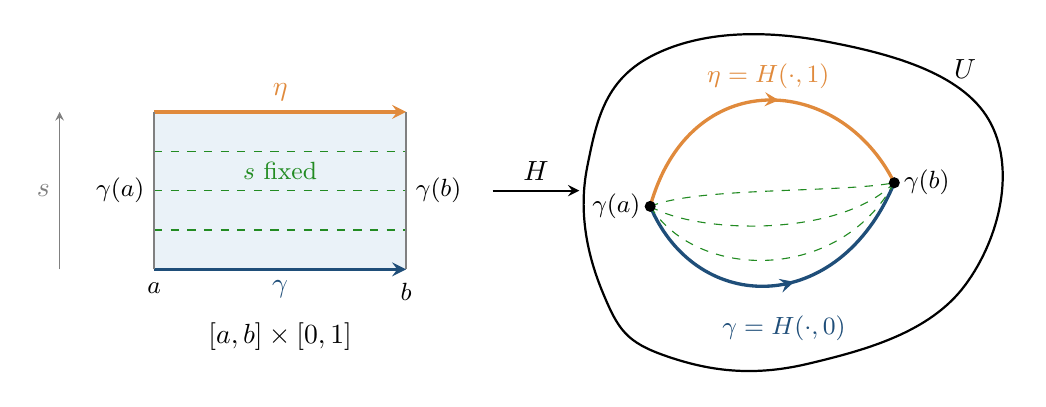
\begin{tikzpicture}[>=stealth,
 decoration={markings,mark=at position 0.55 with {\arrow{>}}}]
 % parameter rectangle
 \fill[lightblue] (0,0) rectangle (3.2,2);
 \foreach \y in {0.5,1,1.5}
  \draw[ForestGreen,thin,dashed] (0,\y)--(3.2,\y);
 \draw[courseblue,very thick,->] (0,0)--(3.2,0) node[midway,below]{$\gamma$};
 \draw[orangeframe,very thick,->] (0,2)--(3.2,2) node[midway,above]{$\eta$};
 \draw[gray,thick] (0,0)--(0,2) (3.2,0)--(3.2,2);
 \node[left,font=\small] at (0,1){$\gamma(a)$};
 \node[right,font=\small] at (3.2,1){$\gamma(b)$};
 \node[below,font=\small] at (0,-0.05){$a$};
 \node[below,font=\small] at (3.2,-0.05){$b$};
 \node[ForestGreen,font=\small] at (1.6,1.25){$s$ fixed};
 \draw[gray,->] (-1.2,0)--(-1.2,2) node[midway,left]{$s$};
 \node at (1.6,-0.85){$[a,b]\times[0,1]$};
 % arrow H
 \draw[->,thick] (4.3,1)--(5.4,1) node[midway,above]{$H$};
 % image in U
 \begin{scope}[xshift=5.9cm,yshift=-0.3cm]
  \draw[thick] plot[smooth cycle,tension=0.7] coordinates
  {(-0.2,0.0) (0.6,-0.8) (2.4,-0.9) (4.4,0.1) (4.7,2.2) (2.6,3.2) (0.4,3.0) (-0.4,1.6)};
  \node at (4.4,2.85){$U$};
  \draw[courseblue,very thick,postaction={decorate}] (0.4,1.1)
   .. controls (1,-0.3) and (2.8,-0.3) .. (3.5,1.4);
  \draw[orangeframe,very thick,postaction={decorate}] (0.4,1.1)
   .. controls (0.9,2.9) and (2.8,2.8) .. (3.5,1.4);
  \foreach \k in {0.45,1.05,1.65}
   \draw[ForestGreen,thin,dashed] (0.4,1.1)
    .. controls (1,-0.3+\k) and (2.8,-0.3+0.95*\k) .. (3.5,1.4);
  \fill (0.4,1.1) circle (2pt) node[left,font=\small]{$\gamma(a)$};
  \fill (3.5,1.4) circle (2pt) node[right,font=\small]{$\gamma(b)$};
  \node[courseblue,font=\small] at (2.1,-0.45){$\gamma=H(\cdot,0)$};
  \node[orangeframe,font=\small] at (1.9,2.75){$\eta=H(\cdot,1)$};
 \end{scope}
\end{tikzpicture}
\end{center}
Horizontal slices map to curves joining $\gamma(a)$ to $\gamma(b)$;
vertical edges collapse to these endpoints. The proof in Lecture~17
used local primitives, compactness, and uniform continuity.

\begin{definition}
A nonempty open set $U\subseteq\C$ is \emph{simply connected} if it is
connected and every closed continuous curve in $U$ is
\emph{null-homotopic in $U$}: it can be deformed within $U$, with its
base point fixed, to the constant curve at that base point.
\end{definition}

\begin{corollary}\label{cor:null}
Let $U\subseteq\C$ be open and $f$ holomorphic on $U$.
If $\gamma$ is a closed continuous curve that is null-homotopic in $U$,
then $\int_\gamma f(z)\,dz=0$.
In particular, this holds for every closed continuous curve when $U$ is
simply connected.
\end{corollary}
\begin{proof}
A null-homotopic curve can be deformed, with its base point fixed, to a
constant curve. The theorem preserves the integral, and a constant
curve has integral zero.
\end{proof}


\section{The local Cauchy integral formula}
\begin{theorem}[Local Cauchy integral formula]\label{thm:cauchy-formula}
Let $D=D(c,R)$, let $U$ be an open set containing $\overline D$, and
let $f$ be holomorphic on $U$. If $z_0\in D$ and
$\gamma(t)=c+Re^{it}$, $0\leq t\leq2\pi$, then
\[
 \boxed{\displaystyle f(z_0)=\frac{1}{2\pi i}
 \int_\gamma\frac{f(z)}{z-z_0}\,dz.}
\]
\end{theorem}

The proof in Lecture~16 hinged on a comparison of integrals over
different circles. Fix $0<r<R-|z_0-c|$ and let $C_r(t)=z_0+re^{it}$,
$0\leq t\leq2\pi$. The outer circle $\gamma$ has basepoint $p=c+R$ and
the inner circle $C_r$ has basepoint $q=z_0+r$. We would like to
establish that for every function $h$ holomorphic on $U\setminus\{z_0\}$,
\begin{equation}\label{eq:circle-comparison}
 \int_\gamma h(z)\,dz=\int_{C_r}h(z)\,dz.
\end{equation}
The issue is that the two circles have different base points:
$p\neq q$, since $|z_0-c|+r<R$. Thus they cannot be homotopic with
fixed endpoints in our sense.

To fix this issue, we consider the straight segment $\alpha$ from
$p$ to $q$:
\[
 \alpha(s)=(1-s)p+sq,\qquad 0\leq s\leq1.
\]


\begin{center}
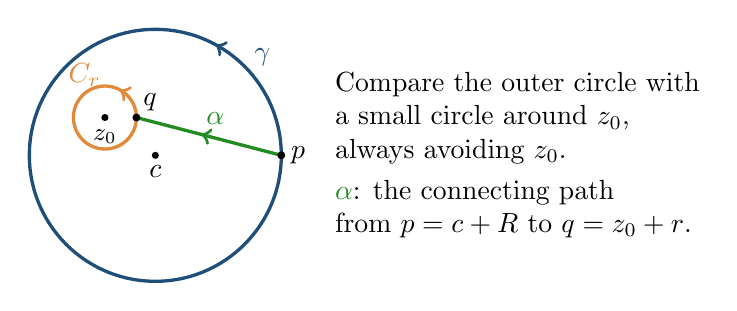
\begin{tikzpicture}[scale=0.8,
 decoration={markings,mark=at position 0.17 with {\arrow{>}}}]
 \draw[courseblue,very thick,postaction={decorate}] (2,0)
 arc[start angle=0,end angle=360,radius=2];
 \fill (0,0) circle (1.6pt) node[below]{$c$};
 \fill (-0.8,0.6) circle (1.6pt) node[below=1pt,font=\small]{$z_0$};
 \draw[orangeframe,very thick,postaction={decorate}] (-0.3,0.6)
 arc[start angle=0,end angle=360,radius=0.5];
 \draw[ForestGreen,very thick,
  decoration={markings,reset marks,mark=at position 0.55 with {\arrow{>}}},
  postaction={decorate}] (2,0)--(-0.3,0.6);
 \fill (2,0) circle (1.8pt) node[right]{$p$};
 \fill (-0.3,0.6) circle (1.8pt) node[above right=-1pt]{$q$};
 \node[ForestGreen] at (0.95,0.58){$\alpha$};
 \node[courseblue] at (1.7,1.55){$\gamma$};
 \node[orangeframe] at (-1.12,1.28){$C_r$};
 \node[right,align=left] at (2.7,0)
 {Compare the outer circle with\\a small circle around $z_0$,\\always avoiding $z_0$.\\[0.3em]
 {\color{ForestGreen}$\alpha$}: the connecting path\\from $p=c+R$ to $q=z_0+r$.};
\end{tikzpicture}
\end{center}


Write $\gamma*\alpha$ for the path that follows $\gamma$ and then
$\alpha$, and similarly for $\alpha*C_r$, assigning each piece half
of $[0,1]$. Both paths run from $p$ to $q$. We now construct a homotopy
between them in $U\setminus\{z_0\}$ with fixed endpoints.


\newpage
Consider the continuous map
\[
 F(t,s)=(1-s)c+sz_0+\bigl((1-s)R+sr\bigr)e^{it},
 \qquad 0\leq t\leq2\pi,\quad 0\leq s\leq1.
\]

Put $d=|z_0-c|<R$. The estimates
\begin{align*}
 |F(t,s)-c|&\leq sd+(1-s)R+sr\leq R,\\
 |F(t,s)-z_0|&\geq(1-s)(R-d)+sr>0
\end{align*}
show that $F$ takes values in $\overline D\setminus\{z_0\}$,
hence in $U\setminus\{z_0\}$. Its bottom and top edges give
$\gamma$ and $C_r$, and both vertical edges give the connecting path:
$F(0,s)=F(2\pi,s)=\alpha(s)$.



\begin{center}
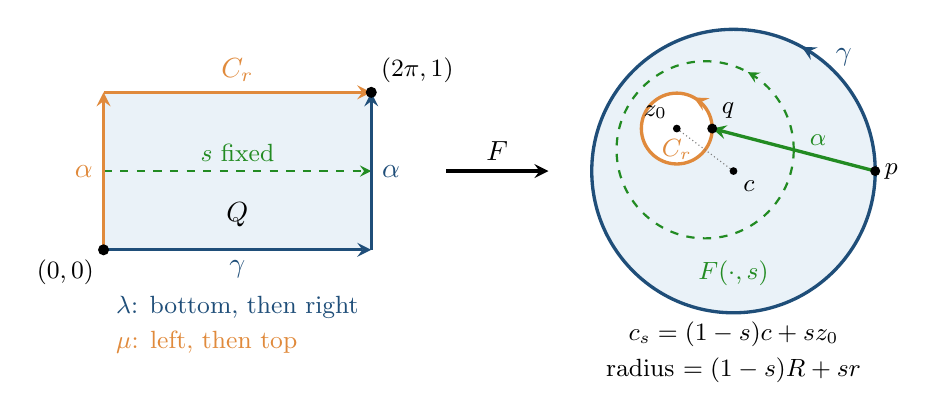
\begin{tikzpicture}[x=1cm,y=1cm,>=stealth,
 decoration={markings,mark=at position 0.17 with {\arrow{>}}}]
 % Parameter rectangle and its two boundary paths.
 \fill[lightblue] (0,0) rectangle (3.4,2);
 \draw[ForestGreen,dashed,thick,->] (0,1)--(3.4,1);
 \node[ForestGreen,above,font=\small] at (1.7,1){$s$ fixed};
 \draw[courseblue,very thick,->] (0,0)--(3.4,0)
  node[midway,below]{$\gamma$};
 \draw[courseblue,very thick,->] (3.4,0)--(3.4,2)
  node[midway,right]{$\alpha$};
 \draw[orangeframe,very thick,->] (0,0)--(0,2)
  node[midway,left]{$\alpha$};
 \draw[orangeframe,very thick,->] (0,2)--(3.4,2)
  node[midway,above]{$C_r$};
 \fill (0,0) circle (2pt);
 \fill (3.4,2) circle (2pt);
 \node[below left,font=\small] at (0,0){$(0,0)$};
 \node[above right,font=\small] at (3.4,2){$(2\pi,1)$};
 \node at (1.7,0.45){$Q$};
 \node[align=left,font=\small] at (1.7,-0.95)
  {{\color{courseblue}$\lambda$: bottom, then right}\\[0.2em]
   {\color{orangeframe}$\mu$: left, then top}};
 % F maps horizontal slices to circles and both vertical edges to alpha.
 \draw[->,very thick] (4.35,1)--(5.65,1) node[midway,above]{$F$};
 \fill[lightblue] (8,1) circle (1.8);
 \fill[white] (7.28,1.54) circle (0.45);
 \draw[courseblue,very thick,postaction={decorate}] (9.8,1)
  arc[start angle=0,end angle=360,radius=1.8];
 \draw[orangeframe,very thick,postaction={decorate}] (7.73,1.54)
  arc[start angle=0,end angle=360,radius=0.45];
 \draw[ForestGreen,dashed,thick,postaction={decorate}] (8.765,1.27)
  arc[start angle=0,end angle=360,radius=1.125];
 \draw[gray,densely dotted] (8,1)--(7.28,1.54);
 \fill (8,1) circle (1.4pt) node[below right,font=\small]{$c$};
 \fill (7.28,1.54) circle (1.4pt)
  node[above left,font=\small]{$z_0$};
 \draw[ForestGreen,very thick,->] (9.8,1)--(7.73,1.54)
  node[pos=0.35,above,font=\small]{$\alpha$};
 \fill (9.8,1) circle (1.8pt) node[right,font=\small]{$p$};
 \fill (7.73,1.54) circle (1.8pt) node[above right,font=\small]{$q$};
 \node[courseblue] at (9.4,2.45){$\gamma$};
 \node[orangeframe,font=\small] at (7.28,1.27){$C_r$};
 \node[ForestGreen,font=\small] at (8,-0.3){$F(\cdot,s)$};
 \node[align=center,font=\small] at (8,-1.3)
  {$c_s=(1-s)c+sz_0$\\[0.2em]
   radius $=(1-s)R+sr$};
\end{tikzpicture}
\end{center}


Let $Q=[0,2\pi]\times[0,1]$, and write
$\lambda,\mu\colon[0,1]\to Q$ for the two boundary paths shown above,
with each edge traversed linearly in half the parameter interval.
The path $\lambda$ follows the bottom and right edges; $\mu$ follows
the left and top edges. The edge labels in the rectangle indicate
the images of the edges under $F$, so
\[
 F\circ\lambda=\gamma*\alpha,\qquad F\circ\mu=\alpha*C_r.
\]

Both paths start at $(0,0)$ and end at $(2\pi,1)$. Since $Q$ is convex,
$\lambda$ and $\mu$ are homotopic in $Q$ with fixed endpoints, e.g.\ by
the straight-line homotopy
\[
 H(t,s)=(1-s)\lambda(t)+s\mu(t),\qquad 0\leq t,s\leq1.
\]
Composing $H$ with $F$ gives a continuous map
$[0,1]\times[0,1]\xrightarrow{H}Q\xrightarrow{F}U\setminus\{z_0\}$,
namely
\[
 C(t,s)=F\bigl((1-s)\lambda(t)+s\mu(t)\bigr),
 \qquad 0\leq t,s\leq1.
\]
This is a homotopy between $F\circ\lambda=\gamma*\alpha$ and
$F\circ\mu=\alpha*C_r$ in $U\setminus\{z_0\}$, with
$C(0,s)=p$ and $C(1,s)=q$ for every $s$.
Thus Theorem~\ref{thm:homotopy}, applied on the open set
$U\setminus\{z_0\}$, and additivity of integrals give
\[
 \int_\gamma h(z)\,dz+\int_\alpha h(z)\,dz
 =\int_\alpha h(z)\,dz+\int_{C_r}h(z)\,dz
 \qquad\bigl(h\in\Hol(U\setminus\{z_0\})\bigr).
\]
Cancelling the connecting-path integrals yields
\eqref{eq:circle-comparison}:
\[
 \int_\gamma h(z)\,dz=\int_{C_r}h(z)\,dz
 \qquad\text{for every }h\in\Hol(U\setminus\{z_0\}).
\]
Applying this to $h(z)=(f(z)-f(z_0))/(z-z_0)$ and to $h(z)=1/(z-z_0)$
justifies both circle comparisons in the proof from Lecture~16, and so
completes the proof of Theorem~\ref{thm:cauchy-formula}.
%
%Apply this to $h(z)=(f(z)-f(z_0))/(z-z_0)$ and $h(z)=1/(z-z_0)$.
%This justifies both comparisons in the preceding proof and completes it.
%
%The same argument compares the concentric circles in the punctured-disc
%example: use $F(t,s)=((1-s)r+s\rho)e^{it}$ and the connecting segment
%$\alpha(s)=(1-s)r+s\rho$. It gives
%$C_r*\alpha\sim\alpha*C_\rho$ with fixed endpoints, and hence
%equal integrals for every function holomorphic on the punctured disc.
%

\section{Primitives on simply connected domains}
% Handwritten Lecture 18, pages 1--3.
We know that a holomorphic function has a primitive on each disc in
its domain, by the Cauchy--Goursat theorem for rectangles in discs.
The homotopy theorem now lets us replace the disc by any simply connected domain.

\begin{theorem}\label{thm:global-primitive}
Let $U\subseteq\C$ be simply connected and let $f$ be holomorphic on
$U$. Then $f$ has a primitive on all of $U$.
More precisely, fix $z_0\in U$ and define
\[
 g(z)=\int_{z_0}^z f(\zeta)\,d\zeta,
\]
where the integral is taken along any continuous curve in $U$ from
$z_0$ to $z$. This is well-defined, and $g'=f$ on $U$.
\end{theorem}

\begin{center}
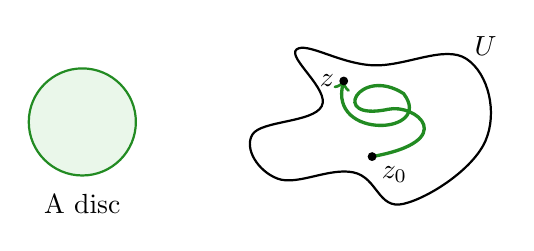
\begin{tikzpicture}[scale=0.8]
 \fill[lightgreen] (-2,0) circle (0.85);
 \draw[ForestGreen,thick] (-2,0) circle (0.85);
 \node[below] at (-2,-1){A disc};
 \begin{scope}[xshift=2.6cm]
  \draw[thick] plot[smooth cycle,tension=0.7] coordinates
  {(-1.5,-0.9) (-1.9,-0.2) (-0.8,0.25) (-1.2,1.15)
   (0,0.9) (1.5,1) (1.8,-0.3) (0.5,-1.3) (-0.3,-0.8)};
  \draw[ForestGreen,very thick,->] (0,-0.55)
   .. controls (1.4,-0.3) and (0.7,0.3) .. (0.25,0.2)
   .. controls (-0.7,0) and (-0.2,0.9) .. (0.5,0.45)
   .. controls (1,-0.2) and (-0.7,-0.3) .. (-0.45,0.65);
  \fill (0,-0.55) circle (2pt) node[below right]{$z_0$};
  \fill (-0.45,0.65) circle (2pt) node[left]{$z$};
  \node at (1.8,1.2){$U$};
 \end{scope}
\end{tikzpicture}
\end{center}

\begin{proof}
\textbf{Existence of paths.} We claim that a connected open subset of $\C$ is
polygonally connected.\footnote{An open set $U\subseteq\C$ is
\emph{polygonally connected} if any two points $z,w\in U$ can be joined
by a \emph{polygonal path} in $U$: a finite chain of line segments
$[w_0,w_1],[w_1,w_2],\dots,[w_{n-1},w_n]$, each contained in $U$, with
$w_0=z$ and $w_n=w$. A polygonal path is piecewise $C^1$, so in
particular it is a continuous curve along which we can integrate.}

Here is a proof using the standard definition of connectedness below.

\begin{remark}[Connected open sets are polygonally connected]
For Theorem~\ref{thm:global-primitive}, we only need that connected open
subsets of $\C$ are \emph{path connected}. The proof below gives the
stronger statement that they are \emph{polygonally connected}.

Call a set $S\subseteq\C$ \emph{connected} if it cannot be split into
two disjoint, nonempty, relatively open pieces. That is, whenever
$S=X\cup Y$ with $X\cap Y=\varnothing$, $X=V\cap S$ and $Y=W\cap S$
for some open sets $V,W\subseteq\C$, then $X=\varnothing$ or
$Y=\varnothing$.

Let $A$ be the set of points of $U$ that can be reached from $z_0$ by a
polygonal path in $U$, and let $B=U\setminus A$.
\begin{itemize}
 \item \emph{$A$ is open.} If $a\in A$, choose a disc
 $D(a,\varepsilon)\subseteq U$. Each $w$ in this disc is reached by
 following a polygonal path from $z_0$ to $a$ and then the segment
 $[a,w]$, which lies in the disc.
 \item \emph{$B$ is open.} If $b\in B$, choose a disc
 $D(b,\varepsilon)\subseteq U$. If some $w$ in this disc were in $A$,
 then appending the segment $[w,b]$ would reach $b$, which is
 impossible. So the whole disc lies in $B$.
\end{itemize}
Thus $U=A\cup B$ is a union of disjoint open sets, and $A\ne\varnothing$
since $z_0\in A$. As $U$ is connected, $B=\varnothing$, i.e.\ $A=U$.
Finally, any two points $z,w\in U$ are joined by following a path from
$z$ back to $z_0$ and then one from $z_0$ to $w$.
\end{remark}

\textbf{Independence of the path.} Suppose $\gamma$ and $\eta$ both
run from $z_0$ to $z$ in $U$. Write $\eta^{-1}$ for $\eta$ traversed
backwards. Then $\gamma*\eta^{-1}$ is a closed curve in $U$.
It is null-homotopic because $U$ is simply connected, so
Corollary~\ref{cor:null} gives
\[
 0=\int_{\gamma*\eta^{-1}}f(\zeta)\,d\zeta
 =\int_\gamma f(\zeta)\,d\zeta-\int_\eta f(\zeta)\,d\zeta.
\]
Thus the definition of $g(z)$ does not depend on the chosen curve.

\begin{center}
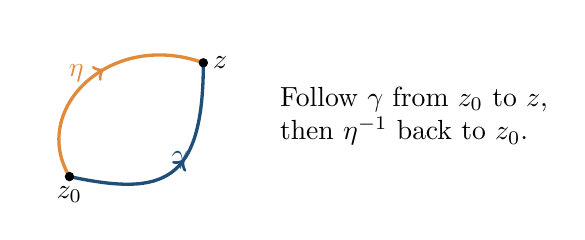
\begin{tikzpicture}[scale=0.85,
 decoration={markings,mark=at position 0.55 with {\arrow{>}}}]
 \draw[courseblue,very thick,postaction={decorate}] (0,0)
 .. controls (1.4,-0.3) and (2,-0.1) .. (2,1.7);
 \draw[orangeframe,very thick,postaction={decorate}] (0,0)
 .. controls (-0.6,1) and (0.6,2.2) .. (2,1.7);
 \fill (0,0) circle (2pt) node[below]{$z_0$};
 \fill (2,1.7) circle (2pt) node[right]{$z$};
 \node[courseblue] at (1.65,0.25){$\gamma$};
 \node[orangeframe] at (0.1,1.55){$\eta$};
 \node[right,align=left] at (3,0.9)
 {Follow $\gamma$ from $z_0$ to $z$,\\then $\eta^{-1}$ back to $z_0$.};
\end{tikzpicture}
\end{center}

\textbf{Differentiating locally.} Fix $z_1\in U$ and choose a disc
$B=D(z_1,\varepsilon)\subseteq U$. Let $G$ be a primitive of $f$ on
$B$. For $z\in B$, use a fixed path from $z_0$ to $z_1$ followed by
the straight segment from $z_1$ to $z$. Path independence gives
\[
 g(z)=g(z_1)+\int_{[z_1,z]}f(\zeta)\,d\zeta
     =g(z_1)+G(z)-G(z_1).
\]
\begin{center}
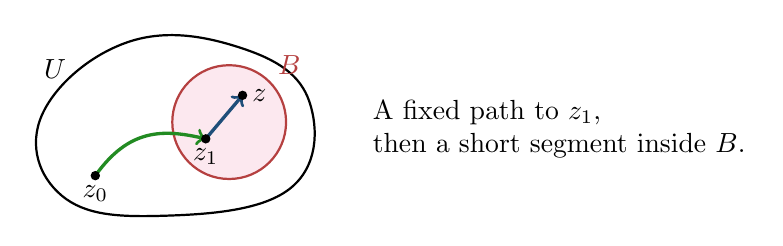
\begin{tikzpicture}[scale=0.85]
 \draw[thick] plot[smooth cycle,tension=0.7] coordinates
 {(-0.5,-0.7) (-0.8,0.5) (0.5,1.6) (2.2,1.5) (3.2,0.7) (2.9,-0.6) (1,-1)};
 \fill[lightpink] (2,0.4) circle (0.85);
 \draw[exerciseframe,thick] (2,0.4) circle (0.85);
 \draw[ForestGreen,very thick,->] (0,-0.4)
 .. controls (0.5,0.3) and (1,0.3) .. (1.65,0.15);
 \draw[courseblue,very thick,->] (1.65,0.15)--(2.2,0.8);
 \fill (0,-0.4) circle (2pt) node[below]{$z_0$};
 \fill (1.65,0.15) circle (2pt) node[below]{$z_1$};
 \fill (2.2,0.8) circle (2pt) node[right]{$z$};
 \node[exerciseframe] at (2.9,1.25){$B$};
 \node at (-0.6,1.2){$U$};
 \node[right,align=left] at (4,0.3)
 {A fixed path to $z_1$,\\then a short segment inside $B$.};
\end{tikzpicture}
\end{center}
The two terms involving $z_1$ are constant as $z$ varies in $B$.
Consequently $g'(z)=G'(z)=f(z)$ on $B$. Since $z_1$ was arbitrary,
$g$ is a primitive on all of $U$.
\end{proof}

\end{document}
